% 从天球的音乐到玻尔模型

\footnote{本文根据 CC-BY 协议转载自季燕江的《量子序曲》, 进行了重新排版和少量修改}形或古希腊人所说的 “idea”,有多种含义,比如:形状,这是和视觉有关的;比如风格、分类,这可以是和视觉有关的,也可以无关,比如音乐也可以有风格,这就是和声音有关的了.

和视觉有关的 “形” 是直观的,我们无须论证,纠结于如何用语言表达,仅凭图形——或者是静态的,或者是想象中动态的——直接给出结果.对形的研究会导向几何学,几何本身是视觉的,而视觉是偏好静的,偏好不动的,但一加 “学”,几何 “学” 或 “学” 几何就动起来了.

我们如何学呢?或者演示,用圆规和直尺,或者像毕达哥拉斯那样拿根木棍面对沙土,世界是一步一步地被展现出来的,一笔一划本身就是个动态的过程.我们努力说: “首先如何,其次如何,然后,又然后……”

所谓动态就是次序,我们首先只关注首先要解决的,其次,带着对刚刚过去的对首先的记忆,探讨紧接着要解决的问题,我们的思想没法分叉.人在专注的状态下,视觉也需要一个焦点.当我们的视觉遭遇挑战,看不清某物的时候,我们凝眼观瞧,把视线使劲聚焦于某物,凝眼就是凝神,不受诱惑地专注于某物,看清楚一点再继续看下一点.

这个结构很像自然数:“0,1,2,3,……”,一步一步地展示给你看,比如 “我是如何用直尺和圆规作图的”,这种线性展开的结构就是时间, “学” 的过程,对学的人是学,在Challenge,对展示的人来说是在 “证”,在说服,这个过程是世界次第展开的过程,是叙事、是 Chronicle.

\subsection{形与声}

“学” 依赖语言,语言是一种声音现象.

据说人能够发出一个八度再加一个四度的声音.

古代世界,天和地很近,音乐和人也很近.孔子闻韶乐 “三月不知肉味”,这种沉浸在声音里的境界和我们今天听流行音乐,把音乐当做一种背景噪音,是完全不同的两种声音技术.今天我们听音乐往往是为了抑制我们心中的背景噪音.

古代的音乐都很简单.简单到好比就是敲击单音音叉发出的声音,单音音叉是校音用的,它在古代世界的对应物是中国的黄钟律管或希腊的单弦琴(Monochord).它们发出很纯的音,基本上就是一个频率.孔子一生关心礼,礼与乐相联,乐就是音及音的混杂与排列.

我们用音高,频率,响度,音色等来描述声音.音高就是频率,是描述 “音” 诸参数中最重要的一个.人天生就是一个感知音高的灵敏动物,高音激越,使人振奋,低音呜咽,让人伤感.简单的音乐庄重使人入静,而复杂多变的音乐也如一场 “视觉的盛宴”,它使我们好奇和沉迷.

听觉和视觉一样,是感觉,同时也是思维,我们的眼睛和耳朵接受信息,同时也处理、歪曲信息以为我们所用.古代的政治传统,古代的教育家都注重音乐教育,这其中最重要的就是对音乐体系的保留和传承.

比如唱歌的时候要先定调,调可以定低点,显得庄重,也可以定高点,显得轻快.定好调后,一系列的声音次第展开,它们的相对音高保持一个固定的结构,比如:

“低,低低,高,高高,低,中中,……”

在给定乐谱的前提下.基准音高的选取,或所谓定调是任意的.我们可以定高点,无非大家唱不上去而已.但因为有人唱不上去,这个定调就也不是完全主观任意的了.

古代政治秩序大多由推崇勇猛进取精神的战士集团建立,对战士共同体而言,最重要的是要保持这种勇猛进取的精神,能够保持这种精神的音乐会与特定音高有关,这是人群的共同经验.比如柏拉图在《理想国》中就说,要摒弃悲伤和软绵绵的吕底亚调和伊奥尼亚调,而推崇多利亚调和佛里吉亚调.

保持这种对声音的共同经验在古代政治传统中是非常重要的,其中之一就是确定音调,或基准音的频率,然后在此基础上给出其他音的定义,其他音是相对于基准音而言的,可以更高,也可以更低,构成一个阶梯状的结构.

原子的 “idea” 是无所不在的,这里由人的听觉经验,我们再次得到了原子的概念,即存在着 “音高” 的原子,进一步细分不同音高的原子是没有必要的.

保存音乐制度最简单的方法就是造一套标准的乐器,然后后人反复向这些标准的乐器学习,第一套自然是由城邦的缔造者 “铸造” 的.

考虑到弦乐器与弦绷紧的程度有关,受湿度、温度影响较大,青铜器制造的发音器会是理想的选择,这是为什么 “钟” 会成为 “国家” 符号的原因,塔可夫斯基电影《安德烈·卢布廖夫》再现的是俄罗斯帝国创旦的精神基础,在影片的结尾就出现了工匠之子铸钟的奇迹.

\begin{figure}[ht]
\centering
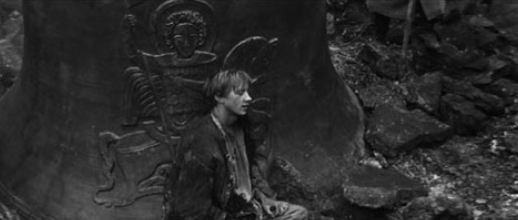
\includegraphics[width=10cm]{./figures/ClBohr_1.png}
\caption{工匠之子铸钟} \label{ClBohr_fig1}
\end{figure}


钟是要发音的,音高是有标准的,“音高” 高一些,低一些,很微妙,但人的耳朵,或某些人的耳朵天生就是辨别音高的灵敏仪器.只有能发出特定音高的钟才是可以被接受,一只发音不准的钟在敲响的时候不嘹亮,不能激发人民激越的精神,这对城邦是不利的.

这里有个似是而非但很有趣的讨论,人有时间感,但人的时间感是非常内在的,几乎不存在什么可以相互交流的基础.这是妨碍人产生运动观念,并研究运动的重要原因.音高即频率,频率就是时间的倒数,人没法准确标记时间的流逝,但人却是辨别频率(时间倒数)的精密仪器.同时我们的发音器官,还能娴熟地对不同音高的声音进行模仿,这是我们具有语言和音乐能力的生物学基础.

类似地,我们还可以讨论视觉,讨论视觉对位置和速度的分辨.人天生就能在相当精确的意义下辨别位置,但我们对速度的判断就要差许多.我们说A比B快,其实是通过位置下的判断,即AB同时出发,但A先撞线,所以A更快.这是亚里士多德无法得到 “正确” 的落体规律的原因,他受人本身的局限,速度是很难直接被看的.

古代实验技术还没有充分发展起来,而实验技术的充分发展与资本主义的生产方式兴盛有关,近代自然科学与资本主义生产方式同步爆发并非巧合.回顾二者,科学史和资本主义发展史,两者讲的是同一个故事,只是叙事的角度生了变化.

由 “造钟” 故事,我们得到一个新洞见,即:“音与形有关”.对钟来说这是大大地简单化了,因为材质也很重要,但形状确实决定了钟振动的频率.这意味着:“听音可以定形,定形可以定音”.

形既是形状也是模型,还是形式.在毕达哥拉斯和柏拉图的传统里,形是与数紧密相连的.比如钟的形由何而定呢?长、宽、高、是数字,钟的厚度也是数字,但这一堆数字的集合又有什么意义呢?

当我滔滔不绝地罗列一堆数字的时候,这是没有意义的.我们需要给出数字和数字之间的关系,才有意义.而且最好是只给出一个关系(或最少关系),就能让所有的数字各就各位.找到这样的规律自然是对思维的奖励,是可以向众人夸耀的;同时这也是技术,有了技术我们就能铸钟,小孩的父亲是会铸钟的,但他把技术带到坟墓里去了.

《安德烈·卢布廖夫》中的小孩是幸运的,他必须试试,他也只能试试.在拜占庭衰败之后,东正教来到了俄罗斯与当地的土豪、愚民混合,文明在绝望中重新开始,这就是俄罗斯的宿命.卢布廖夫受不会铸造但却造出钟的小孩的激励,重新拿起画笔开始画注定会塑造俄罗斯民族精神的那些很平、很抽象圣像画.

\begin{figure}[ht]
\centering
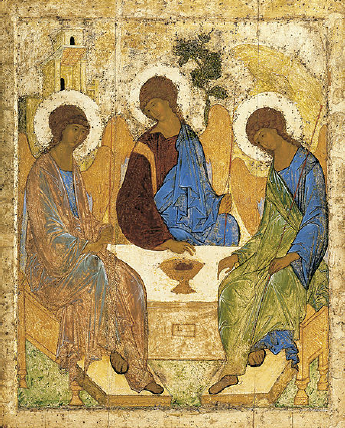
\includegraphics[width=5.5cm]{./figures/ClBohr_2.png}
\caption{卢布廖夫的《三圣像》} \label{ClBohr_fig2}
\end{figure}

画是形(idea),音是声(logos).形和声都能塑造性格,前提是我们生活在某种生活中,或我们生活在某种历史中.

\subsection{数字与和谐}

“几何学”(Geometry)是对形的规定,而 “和声学”(Harmonics)是对音的规定.所谓规定就是数字之间的联系,最简单的数字和数字间的联系是 “相等”,稍微高级点的是比例,是合乎比例.

比如人脸,人脸上五官的位置和尺寸是需要合乎比例的,这种合乎比例是我们天生可以判断的,但很难用数字说清楚.近一二十年随着计算机对数据处理能力的提高和神经科学的进步,在这方面有了很多具体技术的进展.

比例或合乎比例会产生美,这是某种审美观念下的模式识别.比如古代东夷部族以扁头为美,甚至不惜把小孩的头骨弄扁以合乎比例.这个习俗在今天还有遗存,不少地方有端正小孩睡姿以把头睡扁的说法.

在音乐中我们很容易发现音高与数字的关系.这是毕达哥拉斯的贡献.音乐的历史一定很古老.在毕达哥拉斯之前人类就有音乐了,不但有音乐还有规定音高的一套体系,即有一套术语来说清楚“不同音高”的音之间的关系.

比如当我发出一个音后,让你发出一个高四度的音,你就能发出这样一个音,并得到我的认同.这套语言游戏能够玩儿的起来.这些当然都是基于感官经验讲的,本来和数字没啥关系.传说毕达哥拉斯在路过铁匠铺时,受到叮叮当当声音的启发,回去研究各种乐器的音高,比如弦乐.

所谓弦乐器就是一根绷紧的弦,两端固定,中间可以快速振动起来,扰动空气发出声音,弦乐的频率自然就是琴弦发出的声音.这是典型的机械振动的问题,弦上会有波动,但因琴弦两端是固定的,所以波传播不出去,它只能被限制在琴弦上振动,并整体具有一个轮廓,琴弦就在这个轮廓内振动,这种振动叫驻波.

琴弦上的振动是波动,当一列波从左向右传播时碰到弦的端点会反射回来,驻波就是两列相向传播的波的叠加:

\begin{equation}
\frac{A}{2} \left( \cos ( kx - \omega t ) + \cos ( kx + \omega t ) \right) = A \cos kx \cos \omega t
\end{equation}

这里A是振动的幅度,振动的轮廓线是:

\begin{equation}
A \cos kx 
\end{equation}

$k = \frac{2 \pi}{\lambda}$是波矢,$\lambda$是波长,因为琴弦的两端已经被限制住了,琴弦的长度$L$可以取半波长,一个波长,一个半波长,……,简单说就是半波长的整数倍:

\begin{equation}
L = \frac{n \lambda}{2}, n = 1, 2, 3, ...
\end{equation}

波长可以表示为:

\begin{equation}
\lambda = \frac{2L}{n}
\end{equation}

这就是合乎比例.

考虑到弦上波速$v$是个常量,频率可以表示为:

\begin{equation}
\nu = \frac{n v}{2 L }
\end{equation}

给定弦长$L$,只有这样的波动,或这样波动的叠加才可以存在.进一步讲,如果我们考虑一个符合两端被限制住的琴弦的一般运动,这个一般运动总是可以被分解为一系列不同$n$取值的,波长为$\lambda_n = \frac{2L}{n}$,频率为$\nu_n = \frac{n v}{2 L }$的振动的叠加.

\begin{equation}
\sum\limits_{n} A_n \cos \frac{n \pi x}{L} \cos \frac{n \pi vt}{L}
\end{equation}

我们管$n = 1$的音叫做基音,这个频率$\frac{v}{2L}$的声音是最主要的,但弦上也会有$n= 2, 3, ...$的成分,这些音叫做泛音.

拨动长度$L$的琴弦,我们听到的是基因和泛音的混合,最主要的是基因,频率为$\nu_1 = \frac{v}{2L} $,其次是第一个泛音,频率为$\nu_2 = 2 \nu_1$,它们之间是1: 2的关系.

假如我们把琴弦的长度减半,其实就是用手在弦长的一半按住琴弦,此时我们会有新的弦长$L/2$,同时新的基因频率$2 \nu_1$,但此时,因为弦长只剩下一半了,我们拨动琴弦发出的声音里就没有$\nu_1$的成分了.

听起来的感觉是这样的,首先$L/2$琴弦发出的音和$L$琴弦发出的音很像,其次$L/2$琴弦发出的音当然要比$L$琴弦发出的音要高,这就好比是一个人沿螺旋形的楼梯升高,每个台阶都对应一个特定音高的音,在螺旋式升高了几个音之后我们又回到了起始位置,只是高了一些,我们还可以继续螺旋升高,每提升一个台阶都会感觉和曾经的某个台阶很像,只是更高了.

在音乐理论里,我们管这个结构叫 “八度”,当音高由 $\nu_0$ 提高一倍到 $2 \nu_0$ 的时候,我们就说 “升了八度”.类似地,当音高由$nu_0$降一倍到$\nu_0 /2$时,我们就说 “降了八度”.我们一般能发出一个八度再加一个四度的音.

\subsubsection{毕达哥拉斯的和声学}

毕达哥拉斯研究了音和形的关系,并发现这个关系可以被数字精确地描述.比如我们刚刚讨论过的,当弦乐器的弦长比是1:2时,频率比是2:1,正好对应音乐理论中的 “八度音程”.

八度关系本来就存在于音乐实践中,属于人的日常经验.现在发现 “一个八度” 可以表示为精确的数字比1:2,这个数字比其实是对形的描述.只是因为这里弦是一维的,我们对形的描述比较简单.

一个日常经验可以对应于一个数字的比例关系是足够让人兴奋的,毕达哥拉斯讲 “万物皆数”,其实讲的是 “万物皆合乎比例”.只有合乎比例,万物才能存在,只是这些比例有待我们的发现.

合乎比例是个静态的世界观.

除了1:2,毕达哥拉斯还发现当弦长比是2:3时,音的关系是音乐理论中的五度音程.而弦长比是3:4时是音乐理论中的四度音程.毕达哥拉斯只发现了这几个关系.它足够优美,但还不足以解释音乐理论中所有的音.但这已经足够他嘚瑟的了.

更重要的是他开辟了一个用数字、用比例关系去研究音乐的方法,进而是研究整个宇宙万物的方法,可以说今天的理论家都是毕达哥拉斯的信徒.

\begin{figure}[ht]
\centering
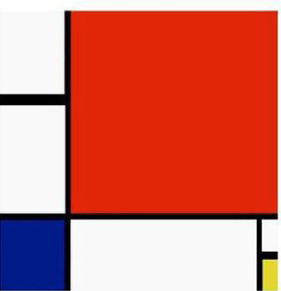
\includegraphics[width=5cm]{./figures/ClBohr_3.png}
\caption{蒙德里安的作品是 “万物皆数”、 “整体和谐” 观念在绘画领域的实践.} \label{ClBohr_fig3}
\end{figure}

毕达哥拉斯方案的缺陷是他被简单数字迷住了,1:2,2:3,3:4确实解释了八度音程、五度音程、和四度音程.但再要想把人对声音的感官经验——极其灵敏的感官经验——和简单数字比(m:n)建立关系就很困难了.

根据近代的十二平均律,我们在八度音程里面做12均分,这个均分是合乎比例地分——作为人,我们当然是凭我们的耳朵来分,这里我们必须赞叹人听觉器官的精密——我们要找到某个合适的比例因子$q$,使得:

$1 \nu_0$,$q \nu_0$,$q^2 \nu_0$,……$q^{12} \nu_0 =2 \nu_0$

因此:

\begin{equation}
q = 2^{\frac{1}{12}}
\end{equation}

这里难的是对2开12次方,$\sqrt{2}$就已经是无理数了,即$\sqrt{2}$就已经没办法表示成一个简单数字的比例了!这是毕达哥拉斯方案失败的原因.

我们解出:$q \approx 1.059463 $,并制表:

\begin{table}[ht]
\centering
\caption{⼗⼆平均律}\label{ClBohr_tab1}
\begin{tabular}{|c|c|}
\hline
n & $q^n$\\
\hline
0 & 1 \\
\hline
1& 1.059463 \\
\hline
2 & 1.122462 \\
\hline
… & … \\
\hline
11 & 1.8877 \\
\hline
12 & 2 \\
\hline
\end{tabular}
\end{table}


四度音程对应的弦长比是3:4,计算出来的频率比是:$\frac{4}{3} = 1.33333$,对应十二平均律表格中是$n = 5$的情形,可见:$1.33484$和$1.33333$相当接近.五度音程对应的弦长比是3:2,频率比是:$\frac{2}{3} = 1.5$,对应十二平均律是$n=7$,$1.49831$和$1.5$也很接近.

\subsection{天体音乐}

音乐与舞蹈相联系,古人总是载歌载舞,而载歌载舞是对 “天”,对想象中 “绝对秩序” 的模仿,通过模仿来表达对 “天” 和人格化的 “天”——神的亲近和虔敬.

根据古人的观念,天是天球,有几重天球,离地球最远的是恒星天,它们构成了一个背景,一个不动的背景.还有行星,“金木水火土,太阳和月亮”,它们相对于不动的背景穿行.每个行星都有自己的天球,以自己独特的方式运动.

天体运行的很慢,在没有灯光污染的古代,天体运行是很合适的研究对象,对恒星而言就是绘制星表,把所有可见的,相对而言都不运动的那些恒星的方位表达出来,所谓方位就是方向,所有恒星离我们是一样远的,它们居于最外层的天球.

在这种叙述下,每个恒星对应一个倾角$\theta $和一个方位角$\phi $,我们需要某种制图技术把天球上的恒星投影到平面上,这种制图技术和制作世界地图的技术没有什么区别.我们得到的星图,简单说就是诸星座.

恒星天以下还有土星天球,木星天球,火星天球,太阳天球,金星天球,水星天球和月亮天球.这是按照由外到内的次序,月亮天球离我们最近,月亮之下就是凡俗世界了(月下世界),万物变化不定,没有规律.但自月亮天球及以上就是神圣的所在,天球庄严地运转,超脱于朽坏和变化,被神圣的数学描述.

数字关系是不朽的,诸天也是不朽的,研究天体运行是研究数学,即像毕达哥拉斯在音乐中曾经找到的,找到简单的比例,天球的运行需要合乎比例,并作为一个整体和谐地存在,所谓和谐就是和声(Harmonics).

这是 “万物皆数”观念在天文学中的运用,古希腊的哲学家们已经能够计算太阳的大小,月球的大小,太阳和地球的距离,以及月亮到地球的距离,各个行星运转的周期等等.在他们的眼里,宇宙整体是一个和谐的存在:诸天各有各的半径,这是宇宙的形,而诸天各以不同的速度运转将会发出声音,速度越快音高就越高,月音低沉,土星离地球最远,运行最快因此土星音也是最激昂的.

传说乐器是阿波罗神给人的礼物,它是理性的象征,乐器因形的合乎比例而发出和谐的声音,和谐的声音使人的心灵柔和、敏感,function well成为一架理性的机器.

据柏拉图的《蒂迈欧篇》,宇宙是造物主理性的设计,在比喻的意义下,我们把宇宙想象为一把里拉琴,诸天的位置对应弦上不同的位置.我们无法想象这天体的音乐是不合乎比例的,虽然我们谁都没有听过天体的音乐(天籁之声),但诸天发出的音乐,有的如男低音,有的如男高音,又有的如女低音,有的如女高音.并整体符合某种比例,某种和谐关系.就好像毕达哥拉斯发现的弦乐中的1:2:3:4.

\begin{figure}[ht]
\centering
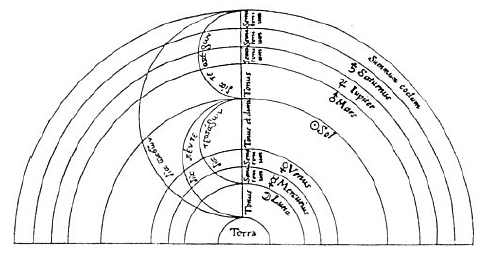
\includegraphics[width=9cm]{./figures/ClBohr_4.png}
\caption{天体音乐的一种构想:最大圆弧表示八度音程,向下是两个四度音程,从地球向上还有个五度音程,并与从恒星天向下的四度音程正好重合.频率比由高到低是:$2: \frac{3}{2} : \frac{9}{8} : 1$.(根据一本中世纪手抄本的插图绘制,收入O. Pederson, M. Pihl: Early Physics and Astronomy, 1974.图6.1)} \label{ClBohr_fig4}
\end{figure}

这里整体和谐的思想是首要的,它或者体现为音乐的悦耳清晰(比如孔子的 “三月不知肉味”),或者干脆就体现为一种数学关系的简单和优美(比如毕达哥拉斯的 “1:2:3:4”).人对音乐的欣赏和想象是可以闭上眼睛进行的,任随自己的思绪伴随着音乐的节奏奔跑,这就摆脱了日常经验对思维的限制,成为一种纯内在的,只与不朽的形式相关的理性思维.

西塞罗在《国家篇》中让西庇阿梦见自己身处宇宙之中,听到:

“由各个天体自身的运动和冲击产生出声音,这种声音是那些按恰当比率严格区别开来的各个不相等的音程划分出来的;它由高音和低音混合而成,将各种不同的和音造成统一的音程;……在处于最高点的星天(恒星天)历程上,那里的运动无比地迅速,就发生尖锐的快速的声音;而月球的历程(那是最低的)则以厚重的声音运动着;”

我们谁都没有听到过天体发出的音乐,西塞罗说这是因为我们从小听习惯了,反而听不见了.毕达哥拉斯的说法更高明,他说除了他自己谁也听不见天体的音乐,毕达哥拉斯说:

“他既不创作也不演奏任何人类演奏的那种竖琴或歌的旋律,而只使用一种神秘的、莫测高深的神圣方法,全神贯注于他的听觉和心灵,使他自己沉浸在流动的宇宙谐音之中.……只有他才能听到并理解这种谐音,以及由这些天体激发起来的和声.”

毕达哥拉斯的高明之处在于点明依靠感官——耳朵——是听不见 “天体音乐” 的,他需要的沉思,即:全神贯注于听觉和心灵,使自己沉浸在流动的宇宙谐音之中.类似地,柏拉图在《理想国》中嘲笑 “仰望星空者” 是观星迷,并摆明他自己研究天文学的方法是几何学.

研究天文学也并非是简单地应用数学-几何学,按照柏拉图的说法,研究是要发现理念,现象被理念(光)照亮,新的理念就是新的形式,就是新的类.换言之就是要发现具有表现力的新的数学-几何学.

西庇阿之梦是西方艺术中的常见母题,往前自然是毕达哥拉斯的 “天体音乐” 和柏拉图的 “厄尔神话”,往后则是比如库布里克的《2001太空漫游》.

影片开始的时候,节奏非常缓慢,人(猿)生活在自然中,直到他们凭视觉洞见了一个抽象的几何形体从天而降,这是对几何学起源的神话式描写.在 “数学-几何学” 光芒的照耀下,镜头一转人类就进入了太空时代.

\begin{figure}[ht]
\centering
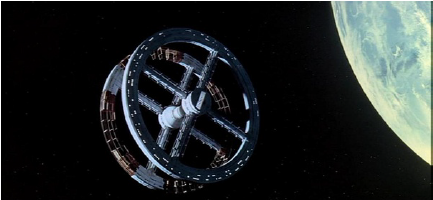
\includegraphics[width=9cm]{./figures/ClBohr_5.png}
\caption{2001 太空漫游} \label{ClBohr_fig5}
\end{figure}


这就是理性的力量,但首先你需要像那只人(猿)一样被理想的几何打动,为之着迷,这就像毕达哥拉斯发现1:2:3:4可以解释音程一样,瞬间被理性的力量击中并宣称 “万物皆数”!

而当影片即将结束的时候,我们看到类似西庇阿之梦的梦境,变换的色彩,抽象的几何形体,流动冲撞,这其实是对天体音乐的视觉再现.而随之进入的是更为具象的人类生活,所有美好或可以激发起美好与和谐感觉的画面,西方历史中值得尊敬和记录的种种视觉切片.

向伟大的西方文明致敬!

从毕达哥拉斯和柏拉图始到太空时代终,影片推出的1968年正是人类进军太空的最高潮,一年后的1969年人类首次登月成功.

在影片即将结束的时候我们听到的是《蓝色多瑙河》.

(从几何形体到《蓝色多瑙河》都是最常见的西方文明的符号.)


\subsection{开普勒}

开普勒是位承前启后的人物,一方面他和托勒密、西塞罗一样醉心于天体音乐的概念,希望能够发现宇宙整体和谐的规律,另一方面他关于行星运动的三个定律直接导致了牛顿的经典力学.

在牛顿的体系里万有引力$F = G M m /r^2$和牛顿第二定律$F = ma$取代了整体和谐,微分和积分取代了数字之间的合乎比例,运动的轨迹取代了静态的天球.

托勒密是古代天文学的集大成者,托勒密天文学的核心是匀速圆周运动,他把行星的运动分解为数个匀速圆周运动的叠加,并很好地与当时的天文学观测数据吻合.这是一种描述性的理论,表面看起来简单,但进入细节后就会觉得很繁复.即便是今天,我们也很难凭脑子去想哪怕是几个匀速圆周运动的叠加.

\subsubsection{开普勒的天球理论}

从整体和谐的观念出发,就需要找到更简单清晰的数学规律,具体说就是某种比例关系.开普勒的出发点和毕达哥拉斯很类似,都是整数.

在开普勒的年代,哥白尼的体系已经逐渐为天文学家接受,太阳不再是行星,地球取代了它的位置.已知行星按距离太阳由近到远排列是:水星、金星、地球、火星、木星和土星.

它们的轨道半径比是:

8:15:20:30:115:195

为什么太阳有 6 颗行星,不多不少正好 6 颗,而它们的半径比又正好是以上的整数比?

今天看来开普勒的问题是完全没有意义的,因为根据万有引力定律,行星实际上可以出现在距离太阳的任何距离上,而今天已知的大小行星的数目也远远超出 6 颗.换句话说,开普勒的问题只有放到 “整体和谐” 观念下才有意义.

柏拉图在《蒂迈欧篇》中曾用四种正多面体与 “水气土火” 四种元素对应,但实际上有五种正多面体,这让人感到很不完美.

现在开普勒把五种正多面体与行星所在的天球对应,具体过程是这样的:

\begin{enumerate}
\item 水星天球在最里面;

\item 在水星天球之外构造一个正8面体,使之与水星天球相切,在正8面体外再构造一个外接球,这个球就是金星天球;

\item 在金星天球外构造一个正20面体,地球天球就在这个正20面体的外接球上;

\item 在地球天球外构造一个正12面体,火星天球就位于这个正12面体的外接球上;

\item 在火星天球外构造一个正4面体,木星天球就位于这个正四面体的外接球上;

\item 最后在木星天球外构造一个正立方体,土星天球就位于这个正立方体的外接球上.
\end{enumerate}

这样我们就用5种正多面体,得到了6个行星天球.根据立体几何,我们可以严格证明只有5种正多面体,现在不多不少各用一次,外接内切得到了正好6个行星天球.而在当时人的知识里,太阳只有6颗行星,不多不少6个天球,每个天球上镶嵌上1颗行星.

更加令人赞叹的是,根据开普勒的天球套天球模型,我们能精确地计算出6个天球的半径比,它们正好是:

8:15:20:30:115:195

误差有,但不大(不超过5\%).

这个结果太完美了,可谓是毕达哥拉斯 “万物皆数” 纲领下的巅峰之作.日后开普勒虽然有更为人称道的行星运动三定律,但他本人仍然最钟爱这个 “整体和谐” 观念下的理论.


\subsubsection{开普勒的行星运动定律}

开普勒的这个 “古典理论” 并没有受到当时学术圈的重视,但他树立了他作为优秀数学家的名声.第谷·布拉赫是当时最了不起的实验家,第谷读过开普勒关于天球的著作,虽然不以为然,但主动寻求与他合作.

第谷积累了当时最丰富的对行星观测的资料(也有恒星的),但仅仅是观测就已经耗费了他一生的精力,现在他预感到他的人生不久了,于是把资料留给一位优秀的数学家——开普勒——期待他能把资料整理出来并有所发现,给他带来名声.

第谷的数据中尤其以火星的数据特别详尽,但当开普勒试图用哥白尼的体系对这些数据进行处理时,却碰到了麻烦.

假设火星沿一个匀速圆周的轨道围绕太阳运动,基于哥白尼理论的计算和第谷的实验数据差别较大.本来这个差距可以通过假设更复杂的圆周运动体系来处理——即假设火星同时参与几个匀速圆周运动——这是托勒密和哥白尼体系中都允许的技巧.

这么做带来的是概念上的简单,即只使用更容易让人理解的匀速圆周运动来模仿行星的运动,但从技术的角度,当面对越来越精确的观测数据的时候就会显得太繁琐,并且是难以想象的.开普勒对此非常不满意,于是开始尝试用更多曲线来模仿行星的运动,而不仅仅是限于匀速圆周运动.

\begin{enumerate}
\item 

开普勒关于行星运动的第一个定律说:行星按椭圆轨道围绕太阳运动,太阳在椭圆的一个焦点上.

轨道当然是一种静态的观点,因为它并不涉及快慢.

我们必须要承认想象一个椭圆轨道,可比要想象哪怕两个匀速圆周运动的叠加容易多了.开普勒的椭圆把我们的想象力从哥白尼和托勒密的几十个正圆中解放出来了.

(哥白尼的学说用34个正圆解释了托勒密需要77个正圆才能解释的天体运动,而开普勒现在只需要7个椭圆\footnote{第7个应该是月球的,月球按椭圆围绕地球运动.}.)

\item

开普勒关于行星运动的第二个定律说:行星在离太阳最近的时候运动速度最快,离太阳最远的时候运动速度最慢.并且可以表示为一个比例关系:

\begin{equation}
r v = R V
\end{equation}

这里$r$表示行星离太阳最近时候的距离,$v$表示此时行星运动的速度;而$R$表示行星离太阳最远时候的距离,$V$表示此时行星运动的速度.

这里有快慢,但仍然采取 “合乎比例” 这一静态观点下的语言(和杠杆定律采用的是相同的语言).如果不看$v$,而看角动量(定义为$\vec J = \vec r \times \vec p$)的话,角动量是不随时间变化的.

\item

开普勒关于行星运动的第三个定律说:行星做轨道运动的半径 $R$ ——严格说应该是 “行星离太阳最近距离” 加 “行星离太阳最远距离” 之和的一半——的立方与行星做轨道运动周期 $T$ 的平方之比是个常数.

即:$\frac{R^3}{T^2} $是个常数.

这其实也是在讲运动要合乎比例,只是这个比例更复杂,涉及了立方和平方,考虑到它对所有的行星都适用,这是个强大的、令人耳目一新的定律.

\end{enumerate}


如此优美普适比例关系的背后一定存在着个解释,就好像毕达哥拉斯的 “1:2:3:4” 关系的背后是关于琴弦振动的理论.

\subsubsection{牛顿的经典力学}

开普勒定律的背后是牛顿的经典力学.我们现在来勾勒其轮廓:

\begin{enumerate}
\item 

物体不受外力时,物体将保持匀速直线运动或静止状态.

\item

物体运动状态的改变正比于物体所受的外力之和,反比于物体本身的质量.即:

\begin{equation}
F = ma
\end{equation}

这里质量$m$被定义为物体维持运动状态难易程度的量度.

“物体运动状态的改变” 就是 “物体的加速度”:

\begin{equation}
a = \frac{d v}{d t} = \frac{d^2 x}{d t^2}
\end{equation}

\item

两个具有质量的物体之间会有万有引力,万有引力正比于两个物体质量的乘积,同时反比于两物体间距离的平方.

\begin{equation}
F = \frac{G M m}{r^2}
\end{equation}

假设A、B之间存在引力相互作用,A给B多大的力,B就给A多大的力,只是方向反了.

\end{enumerate}

仔细读的话,这里有两种定义质量的方式,一种是通过运动定义的,物体保持原运动状态的难易程度,叫惯性质量;另一种是通过引力定义的,叫引力质量.我们假设引力质量和惯性质量是相同的,这里并没有太多道理可讲,或者看做是实验(比如落体实验)的结果(同时落地),或者干脆讲这就是个假设,一个迄今不会给理论带来麻烦的假设,不但不会带来麻烦,还会带来好处,比如它是研究广义相对论的出发点.

牛顿的体系和古典的 “天球音乐” 模型相比差距很大.在牛顿的体系里力是核心概念,力驱动行星运动,相比于太阳,行星很小,我们可进一步把行星抽象为具有质量的点(mass point,质点),它在万有引力的驱动下运动.

我们要想了解行星的运动,需要发展求解微分方程的技巧,即如何求解:

\begin{equation}
F=ma
\end{equation}


这是一个关于位置$x(t)$的二阶微分方程,所谓二阶就是这里出现了对时间$t$的二阶微分$\frac{d^2 }{ dt^2 }$.我们需要积分一次求出速度如何随时间变化$v(t)$,然后再积分一次求出位置如何随时间变化$x(t)$,最后再根据$x(t)$得到行星运动的轨迹,比如一个椭圆.

轨迹是整体、静止观念下的,但为了得到轨迹,我们必须由力$F$而$v(t)$,再$x(t)$.从数学的角度,这当然要比列等式,加减乘除、乘方、开方要难.并且这里真正具有运动的概念了,或者说变化,时时刻刻的变化是个逃不掉的概念.

这可以从对速度的定义看出:

\begin{equation}
v = \frac{d x }{d t} = \lim\limits_{\Delta t \to 0} \frac{\Delta x}{\Delta t}
\end{equation}

如果仅仅把速度定义为:

\begin{equation}
v = \frac{\Delta x}{\Delta t} = \frac{ x(t_2) - x(t_1) }{ t_2 - t_1 }
\end{equation}

这还是一个静态的图像,即我们在时刻$t_2$和时刻$t_1$各拍摄一张快照,分别凝神观瞧,用尺子做测量,然后代进公式里计算.我们怎么说这个速度$v$才不过分?它不属于$t_2$,也不属于$t_1$,它是$t_1$到$t_2$之间的平均效果.

那我们还能说时刻$t_0$时的速度$v(t_0)$吗?如果不能加速度$a$的定义就成了空中楼阁.

在牛顿的体系里,速度必须对每一个点都有意义,但如果我们把眼光只聚焦在一点上是不可能有速度的,速度是变化,对一个点怎么能说变化呢?此时我们考虑的是一个点,但这一点的近邻也必须包括进来,否则就不会有变化,不会有速度.

记号:$\lim\limits_{\Delta t \to 0} \frac{ x(t + \Delta t) - x(t) }{\Delta t}$ 表示的是一系列的操作,我们先测$\Delta t = 1$秒,然后0.1秒,0.01秒,0.001秒……

如此构造出一个无穷的序列,就像我们曾经讨论过的0,1,2,3……,这是一个用自然数标记的序列,它是可数的(countable),但无限延伸,没头儿.从技术的角度,我们会发现这个序列往往会很快收敛在某个稳定值上,这个就叫极限.


某时刻 $t_0$ 的速度 $v(t_0)$ 因此就有了定义,它是在极限下得到定义的,这个极限可能存在,可能不存在,但我们物理上只讨论那些极限存在的情况.所谓微积分就是要发展出一套这么做的技巧,更重要的是逻辑体系,把它说严谨,用公理、定义和定律的体系.

现在我们就有了经典力学.

\subsection{原子光谱的玻尔理论}

\subsubsection{经典电磁学}

经典力学里有一条不太让我们放心,这里面似乎只有引力,而引力是个太弱的力.两个人面对面站着,吹口气的力都比他们之间的引力大.

在我们的生活中,除重力外,其他力基本上都不是引力,比如弹簧的弹性回复力,比如我们俩亲切地抱着的压力,比如摩擦力……

这些力的来源是电磁相互作用.

电现象、磁现象和光现象都是人类很早就发现并研究的现象.其规律被麦克斯韦总结成一组非常优美也抽象的数学公式(麦克斯韦方程组):

\begin{equation}
\begin{aligned}
\div E & = \frac{\rho}{ \epsilon_0}\\
\div B & = 0 \\
\curl E & = - \frac{\partial B}{\partial t} \\
\curl B & = \mu_0 j + \mu_0 \epsilon_0 \frac{\partial E}{\partial t}
\end{aligned}
\end{equation}


\begin{enumerate}
\item 

这里第一个式子说的事情和引力很类似,写成力的形式:

\begin{equation}
F = \frac{1}{4 \pi \epsilon_0} \frac{q_1 q_2}{r^2}
\end{equation}

即两个电荷之间的力与电量的乘积$q_1 \cdot q_2$成正比,与两个电荷之间距离的平方$r^2$成反比.

这个结果和万有引力几乎一模一样,有两点不同:(1)我们这里讨论的静电力(也叫库仑力)比引力要强的多;(2)有两种电荷,相同电荷之间是斥力,而相异电荷之间是引力.

\item

第二个式子说的是,在自然界中不存在磁单极子,但物理学家早就准备好了一套磁单极子存在的理论了,只等哪天找到它,就在方程的右侧加上一项.

\item

第三个式子和第四个式子说的是变化的磁场会感生电场,而变化的电场也会感生磁场;前者是发电机的原理,而后者是电磁铁的原理.它们在一起可以解释电磁辐射或光波的存在.

\end{enumerate}

在电磁学的研究中,由于电磁相互作用太强了,力反而不是重点,重点是场,是电场和磁场在时空中的分布和传播.比如对一个电的振子,能量会以电磁波的形式向外辐射,这是必须考虑的物理过程.而对引力,我们就根本不需要考虑引力波.

\subsubsection{经典理论的困难}

假设一个质子和一个电子,相距$0.5 \times 10^{-10}$米,这个距离就是氢原子中电子和质子的距离.我们可以先计算他们之间的电磁相互作用,电子和质子都带一个单位的电荷$e$,但符号相反电子带负电,质子带正电.

\begin{equation}
F_e = - \frac{1}{4 \pi \epsilon_0}\frac{e^2 }{r^2 }
\end{equation}

这里:真空电容率,$\epsilon_0 = 8.854 \times 10^{-12} F \cdot m^{-1}$;电子电荷,$e = 1.602 \times 10^{-19} C$.代入计算得:

\begin{equation}
F_e = 8.25 \times 10^{-8} (N)
\end{equation}

看起来很小,但要看和谁比.

现在计算电子和质子之间的万有引力,还是这个间距,

\begin{equation}
F_g = \frac{G m_e m_p }{r^2}
\end{equation}

这里:引力常数,$G = 6.673 \times 10^{-11} N \cdot m^2 / kg^2 $;电子质量,$m_e = 9.109 \times 10^{-31} kg $;质子质量,$m_p = 1.673  \times 10^{-27 } kg  $.代入计算得:

\begin{equation}
F_g = 3.63 \times 10^{-47} (N)
\end{equation}


电磁相互作用和引力的比值是:

\begin{equation}
\frac{F_e}{ F_g } = 2.27 \times 10^{39}
\end{equation}

电磁相互作用要远远大于引力.

这意味着引力对研究原子尺寸的物理问题是完全可以忽略不计的.

现在只考虑电磁相互作用,电磁相互作用使电子围绕质子运动,但电子会向外辐射电磁波,它损失能量的速度太快了,电子会飞快地撞向质子.估算的结果是只需要$10^{-11}$秒数量级的时间电子就会掉到质子上,即氢原子是不稳定的.

它只能在这个世界上存在一瞬,但经验告诉我们,我们身体里有大量的氢原子,而我们是稳定的.

这就是把经典理论应用到原子现象时碰到的困难.

\subsubsection{氢原子光谱}


一个成功的原子理论应该能够描述原子物理学中的典型现象,原子是稳定的存在,这当然是其中很重要的一个现象.但除此之外还有更独特地属于原子的现象——光谱现象.

光谱现象分为两类,发射光谱和吸收光谱.

所谓发射光谱就是炙热原子发射的光通过三棱镜分光形成的谱分布,吸收光谱是当热光源发出的光通过冷原子气体时,部分光被原子吸收后形成的谱分布.所谓谱分布就是光强相对于波长的分布.

\begin{figure}[ht]
\centering
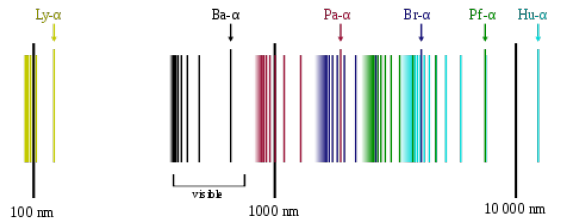
\includegraphics[width=10cm]{./figures/ClBohr_6.png}
\caption{氢原子光谱} \label{ClBohr_fig6}
\end{figure}


我们发现发射光谱中原子发出的特定波长的光,在吸收光谱中也出现,只不过发射变成了吸收.

通俗地说原子就是一个爱戴戒指的人,但她只戴特定尺寸的戒指,戴腻了她就扔,扔掉戒指的尺寸和她拿来戴的尺寸完全一样.对这个现象的解释倒也简单,因为她有5个手指,每个手指粗细不同,但都有确定的尺寸.

我们有理由猜测光谱与原子的本性有关,实验也确实支持我们的这种想法,每种原子都有不同的光谱,它们的谱线出现在不同波长的位置上,就好像是指纹,人人不同,成为我们的标识.

即便是对最简单原子的光谱,比如氢原子的光谱,乍看起来都是很复杂的,但感觉它们是有规律的,或用老话讲,看起来它们是合乎比例的,只是这个比例有待我们的发现.

就好像毕达哥拉斯发现和声学里的1:2:3:4,原子物理早期的突破也来自于人们找到了一个简单、优美的数学式子,这个式子解释了氢原子光谱中可见光区域里的谱线位置(即巴尔末系):

\begin{equation}
\frac{1}{\lambda} = \frac{4}{B} \left( \frac{1}{2^2} - \frac{1}{n^2} \right)
\end{equation}

其中$n = 3, 4, ...$,这就是巴尔末公式,它解释了氢原子光谱中最显著的几条线,很快被推广为里德堡公式:

\begin{equation}
\frac{1}{\lambda} = R_H \left(  \frac{1}{n^2} - \frac{1}{n'^2}  \right)
\end{equation}

这里 $n = 1,  2, ...$,$n' = n+1, n+2, ...$.

里德堡公式可以解释氢原子光谱中所有的谱线位置.

原子的稳定性仍然是很重要的问题,但现在首先要解释为什么会有谱线的规律,这个简单的公式强烈地提示我们在氢原子的问题里存在着更为简单清晰的概念体系和数学结构.

\subsubsection{玻尔理论}

%玻尔理论是导致量子力学出现的关键环节,

某种意义上说,玻尔理论从牛顿的经典力学重新退回到了毕达哥拉斯的 “天球音乐” 图像.天球之所以只奏响这些特定的音,是因为整体的和谐,是形的制约,使天球只能发出特定音高的音.

现在氢原子就是个小天球,它只发射(或吸收)特定波长的光,特定波长的光就是特定频率的光,频率(音)是 “形” 制约的结果,形的制约就是几何关系,两端固定的弦就是一维振动的形.现在我们需要发现的是氢原子的形.

首先这里有个概念需要澄清,我们说是说氢原子,但其实这里我们研究的是电子,因为质子比电子质量大太多了,质子运动的速度比电子运动的速度要小很多,或者说质子很难跟得上电子的运动,所以我们这里只需要研究电子的运动就可以了,而质子则作为固定的背景最后考虑.

现在假设有一个毕达哥拉斯的信徒来研究原子中电子的运动,他会怎么说呢?

首先电子仍然会受质子的吸引,这个力是:

\begin{equation}
F = \frac{1}{4 \pi \epsilon_0} \frac{e^2}{ r^2 }
\end{equation}

假设电子处在某个半径为$r$的正圆轨道上,电子的势能是:

\begin{equation}
V(r) = - \frac{1}{4 \pi \epsilon_0} \frac{e^2}{ r }
\end{equation}

电子的动能是:

\begin{equation}
K = \frac{1}{8 \pi \epsilon_0} \frac{e^2}{ r }
\end{equation}

电子的总能量是:

\begin{equation}
E = K + V = - \frac{1}{8 \pi \epsilon_0} \frac{e^2}{ r }
\end{equation}

电子只能在特定的轨道上运动,这就好像毕达哥拉斯派把宇宙想象为一把里拉琴,只允许在能奏响整体和谐乐音的位置上放置天球,行星在天球上沿正圆轨道呼啸而过,发出特定频率的声音,行星的速度越快,频率也越高……

现在我们只需要把这幅图像套用过来即可,电子也只能出现在特定半径的轨道上,到底是哪些半径允许,这是有标准的,类似于弦上驻波的整体和谐的标准.

%%%%%%%%%

但电子怎么能和波联系起来呢?假如要联系起来又应该怎么联系呢?

硬要往下讲就是假想的历史了.因为玻尔确实不是按这个思路思维的,而德布罗意提出物质波又在玻尔之后,受玻尔模型的启发.

我们现在要求自己有如神助,假想一个能代表电子和谐运动的波沿着电子的轨道运行,运转一圈正好是波长的整数倍,首尾相接形成圆轨道上的驻波.

\begin{equation}
2 \pi r = n \lambda
\end{equation}

我们又想到行星运转越快对应发出的声音就越高,频率$\omega = 2 \pi /T$是时间上的调制,还有波矢$k = 2 \pi / \lambda$,反映的是空间上的调制.

假如我们让电子运行的速度乘以质量(即动量)正比于波矢$k$会有什么结果呢?(纯属猜测)

假设比例因子是$\hbar$,这个比例因子是研究原子尺度物理问题必须出现的.

\begin{equation}
p = m v = \hbar k = \hbar \frac{2 \pi }{\lambda}
\end{equation}

因此:

\begin{equation}
m v r = \hbar \frac{2 \pi r}{\lambda} = \hbar \frac{ n \lambda }{ \lambda} = n \hbar
\end{equation}

即:

\begin{equation}
mvr = n \hbar 
\end{equation}

这就是我们猜测出的对氢原子而言,整体和谐的条件.

电子只能处在由$mvr=n \hbar$(角动量量子化条件)规定的$r$上,并满足:

\begin{equation}
\frac{m v^2}{2} = \frac{1}{2} m \left(  \frac{ n \hbar  }{ m r }  \right)^2 = \frac{1}{8 \pi \epsilon_0 } \frac{e^2 }{r }  
\end{equation}

求得:

\begin{equation}
r_n = n^2 \frac{4 \pi \epsilon_0 \hbar^2  }{ m e^2}, n = 1, 2, 3, ...
\end{equation}

定义玻尔半径$a_0$为:

\begin{equation}
a_0 = \frac{4 \pi \epsilon_0 \hbar^2  }{ m e^2}
\end{equation}

$r_n = n^2 a_0$(代入物理常数,可计算得$a_0 = 0.529 \times 10^{-10} m$),由这一系列$r_n$,我们可以得到一系列的能量$E_n$:

\begin{equation}
E_n = - \frac{m e^4 }{ 32 \pi^2 \epsilon_0^2 \hbar^2 } \cdot {\frac{1}{n^2}}
\end{equation}

或代入具体数值:

\begin{equation}
E_n = \frac{-13.6 eV}{n^2}
\end{equation}

因为整体和谐条件的限制,电子只能占据那一系列轨道$r_n$,因此能量的取值也是一系列分立的取值$E_n$,这一系列分立取值的电子能量就叫做能级.电子离质子越近(n小),电子的能量越低,反之电子离质子越远(n大),电子的能量就越高.

氢原子里只有一个电子,假设这一个电子处在比较高能量的轨道上,它可以向下跃迁,电子的能量将降低,多余的能量将以光子的形式释放出去,假设较高能级用$n'$标记,较低能级用$n$标记,能量差为:

\begin{equation}
h \nu = \frac{hc}{\lambda} = E_{n'} - E_n = 13.6 \times \left( \frac{1}{n^2}  - \frac{1}{n'^2} \right) eV 
\end{equation}

于是我们得到里德堡公式.

\begin{equation}
\frac{1}{\lambda } = \frac{13.6 eV}{hc} \times \left( \frac{1}{n^2}  - \frac{1}{n'^2} \right)
\end{equation}

原子的稳定性还是问题吗?在整体和谐的观念下其实已经没有问题了.我们急需澄清的是那个与电子的运动状态相联系的波到底是什么?此刻——玻尔模型的出现——说明替代范式已经出现,与其苦苦执着于老范式,不如发展新范式,而在新范式下,很多老问题是没有意义的,它们被更急迫的问题所替代.

\begin{exercise}{}
考虑一个平面版的开普勒 “圆环套圆环模型”,最内层是个圆轨道,比如水星,然后在外面套一个正方形,使正方形的四条边与水星轨道相切,然后再在正方形的外面再外接一个圆,作为金星的轨道.我们在金星的轨道外做一个正三角形,使正三角形的三条边与金星的轨道相切,最后在金星的轨道外面做一个外接圆,是地球的轨道.

现在我们可以求出水星轨道、金星轨道和地球轨道的比值了,并与观测数据进行比较.
\end{exercise}

\begin{exercise}{}
下表罗列了开普勒时代六大行星的轨道和周期,你能否把六大行星的轨道比表示为简单整数比,并计算这么做的误差是多少.

\begin{table}[ht]
\centering
\caption{六大行星的轨道和周期}\label{ClBohr_tab2}
\begin{tabular}{|c|c|c|}
\hline
行星 & 轨道半径(天文单位) & 周期(年) \\
\hline
水星 & 0.387 & 0.24  \\
\hline
金星 & 0.723 & 0.615 \\
\hline
地球 & 1.0 & 1.0 \\
\hline
火星 & 1.524 & 1.88 \\
\hline
木星 & 5.2 & 11.86 \\
\hline
土星 & 9.539 & 29.46 \\
\hline
\end{tabular}
\end{table}
\end{exercise}

\begin{exercise}{}
下图是古希腊时期的音阶图,包含两个八度和一个四度,试计算出各个频率比.同时我们也发现某些音是无法根据毕达哥拉斯的 “1:2:3:4”规律计算的.这构成了音乐理论中的一个问题,即如何把剩下音的规律用数字表达出来.

\begin{figure}[ht]
\centering
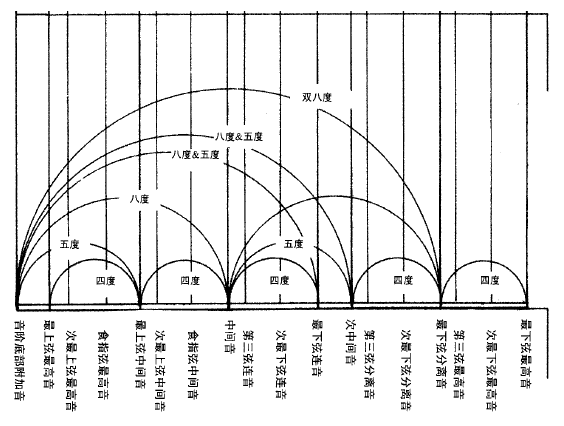
\includegraphics[width=12cm]{./figures/ClBohr_7.png}
\caption{和声的基本原理:音阶.(维特鲁威,《建筑十书》,北京大学出版社,2012.图81)} \label{ClBohr_fig7}
\end{figure}
\end{exercise}
